\documentclass[a4paper, 11pt]{article}

\setcounter{tocdepth}{3}
\setcounter{secnumdepth}{3}

\usepackage{comment} % enables the use of multi-line comments (\ifx \fi) 
\usepackage{lipsum} %This package just generates Lorem Ipsum filler text. 
\usepackage{fullpage} % changes the margin
\usepackage[utf8]{inputenc}
\usepackage{gensymb}
\usepackage{graphicx}
\usepackage{booktabs}% http://ctan.org/pkg/booktabs
\usepackage{makecell}
\usepackage{tabularx}
\usepackage[table]{xcolor}
\usepackage{array}
\usepackage{wrapfig}
\usepackage{subcaption}
\usepackage{csquotes}
\usepackage{lscape}
\usepackage{afterpage}
\usepackage{geometry}
\usepackage{listings}
\usepackage{chngcntr}
\usepackage{multicol}

\counterwithin{figure}{section}

\geometry{a4paper, margin=1in}
\renewcommand{\figurename}{Abb.}
\renewcommand{\tablename}{Tabelle}
\newcommand{\code}[1]{\texttt{#1}}

\renewcommand*{\thead}[1]{\bfseries #1}

\renewcommand{\contentsname}{Inhalt}
\renewcommand{\listfigurename}{Abbildungsverzeichnis}


\begin{document}
 
\title{Einführung in die Internationalen Beziehungen - HS2018}
\author{Alex Neher}
\maketitle

\tableofcontents
\newpage
\listoffigures
\newpage

\graphicspath{{./Pictures/}}


\section{Definitionen}
\subsection{Politikwissenschaft}
Die Definition der Politikwissenschaften hat sich mit der Zeit verändert:
\begin{description}
    \item[Traditionell:] Handlungen des Staates und seiner Organe verstehen
    \item[Modern:] Breites Verständnis des Politischen aneignen
    \item[Heute:] Das Zusammenspiel zwischen Staat und Gesellschaft verstehen
\end{description}        

\vspace{10px}
\noindent Die heutige Politiwissenschaft lässt sich in verschiedene Subkategorien unterteilen:
\begin{multicols}{2}
    \begin{itemize}
        \item Das Politische System
        \item Vergleichende Politikwissenschaften
        \item Internationale Beziehungen
\columnbreak
        \item Politische Theorie
        \item Methodenlehre
        \item Politisches Verhalten
    \end{itemize}
\end{multicols}

Man geht davon aus, dass jeder Bürger zumindest ein Grundverständnis der Politik und der politischen Zusammenhänge hat. Der Unterschied zwischen diesem Grundwissen (Allgemeinwissen) und der Politikwissenschaft ist, dass die Politikwissenschaft \textit{auf systematische Art und Weise logisch konsistente, falsifizierbare und gleichzeitig empirisch bestätigte} Aussagen erarbeitet, während es auch als politisches Allgemeinwissen aufgefasst werden kann, wenn man sagt "Hillary Clinton hätte die Präsidentschaftswahl gewonnen, wenn man sich nicht auf die E-Mails konzentriert hätte." Denn diese Aussage ist weder falsifizierbar (man weiss nicht, ob es tatsächlich stimmt) noch ist sie empirisch bestätigt (es gibt keine Referenzwerte, die diese Aussage bestätigen oder eben falsifizieren würden)

\vspace{10px }

\noindent Es gibt \textbf{vier} Kriterien der politikwissenschaftlichen Forschung: 

\begin{description}
	\item[Inferenz: ] Schlussfolgerung über den Einzelfall hinaus. \\
	Ein Einzelfall ist nichts wert. Es müssen möglichst viele Beobachtungen präsentiert werden, die diese These unterstützen.
	\item[Methodik: ] Der Unterschied zwischen wissenschaftlichen Aussagen und Meinungen ist, dass bei Meinungen die Methode nicht zwingend nachvollziehbar (oder überhaupt vorhanden) sein muss, während bei wissenschaftlichen Aussagen die verwendete Methodik öffentlich zugänglich und nachvollziehbar sein muss.
	\item[Verwandte Methodik: ] Wissenschaftliche Aussagen sollten wenn immer möglich mit einer bereits verwendeten und 'anerkannten' Methodik durchgeführt werden, was auch die Nachprüfung der Aussage vereinfacht.
	\item[Schlussfolgerungen: ] Schlussfolgerungen sind zwar unsicher, der Grad/das Ausmass der Unsicherheit ist jedoch abschätzbar \\
	Man kann zwar nicht mit Sicherheit sagen, dass der neue Präsident mit exakt 80\% Wähleranteil gewählt wird, aber man kann davon ausgehen, dass es 80\% $\pm$ 5\% sein wird.
\end{description}

\subsection{Theorie vs. Modell}

\begin{tabularx}{\textwidth}{XX} 
	\textbf{Theorie} &  \textbf{Modell}\\ 
		\blockquote{Abstrahierende und verallgemeinernde Betrachtung und Auseinandersetzung mit der Wirklichkeit} & \blockquote{Eine Vereinfachte Darstellung der Wirklichkeit, um wesentliche Dinge besser zu verstehen} \\
		  & Eine Menge von vereinfachenden Annahmen und daraus ableitbaren Aussagen über einen Zusammenhang \\ 
\end{tabularx}

\vspace{10px}

So kann ein Modell z.B. eine Karte sein: Sie zeigt eine vereinfachte Darstellung der Wirklichkeit (Die Welt, vereinfacht in 2D). Ausserdem werden nur die wichtigen Dinge wie z.b. der Bahnhof dargestellt, während unwichtige Dinge weggelassen werden. 

\paragraph{Arten von Theorien} \mbox{}\\
Es wird zwischen drei Haupttypen von Theorien unterschieden: 

\begin{description}
	\item[Deskriptiv: ] \textit{Was ist das Wesentliche eines Phänomens?} \\
	"Was macht die Staatenwelt aus?"
	\item[Normativ: ] \textit{Wie sollte eine ideale Welt aussehen?} \\
	"Hat die NATO das Recht zur Intervention in souveränen Staaten?"
	\item[Empirisch-analytisch: ] \textit{Wie sieht die tatsächliche Welt aus?} - Fokus auf Erklärung politischer Prozesse/Events \\
	"Wieso hat Trump die US-Wahlen gewonnen?"
\end{description}

\vspace{10px}

Theorien bestehen immer aus \textbf{vier} Bausteinen: 

\begin{itemize}
	\item Akteure und Dispositionen
	\item Strukturen und Strukturwirkung
	\item Prozesse und Interaktionen
	\item Rückwirkung und Dynamiken
\end{itemize}


\vspace{10px}

\noindent Eine Theorie ist nicht immer zwingend eine \textit{gute} Theorie. Gute Theorien erfüllen folgende Kriterien

\begin{description}
	\item [Logische Konsistenz] Die Theorie sollte sich nicht selbst widersprechen und sollten möglichst wenig Interpretationsspielraum bieten.
	\item [Kausale Ketten] Mehrere zeitlich aufeinanderfolgende Ereignisse oder Zustände, die in ihrer Kombination einen bestimmten Effekt hervorrufen $\rightarrow$  Dominokette
	\item [Unidirektional] Eine gute Theorie funktioniert nur in eine Richtung. Vom Zielzustand lässt sich nicht auf den Anfangszustand schliessen.
	\item [Generalisierbar] Mit der gleichen Methodik sollten für ähnliche oder gleiche Theorien ähnliche oder gleiche Resultate erzielt werden.
	\item [Nicht Tautologisch] "Kräht der Hahn auf dem Mist, so ändert sich das Wetter oder es bleibt wie es ist" $\rightarrow$ immer wahr $\rightarrow$ Tautologisch
	\item [Empirisch überprüfbar (falsifizierbar)] "Wenn Bush nicht Präsident wäre, wäre nun Frieden im Nahen Osten" $\rightarrow$  Nicht falsifizierbar
\end{description}

\subsection{Hypothese}

Eine Hypothese beschreibt den Zusammenhang zwischen mindestens zwei Variablen. Es muss mind. eine unabhängige und eine abhängige Variabel geben. Eine Hypothese muss, gleich wie eine Theorie, empirisch falsifizierbar sein. Ebenfalls muss eine empirische Varianz auf der abhängigen und der unabhängigen Variable vorhanden sein.

Eine Hypothese kann man grundsätzlich mit der Formel \textit{Wenn/Je [...] Dann/Desto} aufstellen. (Je reicher ein Staat, desto demokratischer ist es. Wenn ein Staat Meeranschluss hat, dann hat er eine Handelsflotte)

\begin{wrapfigure}[12]{R}{0.5\textwidth}
	\centering
	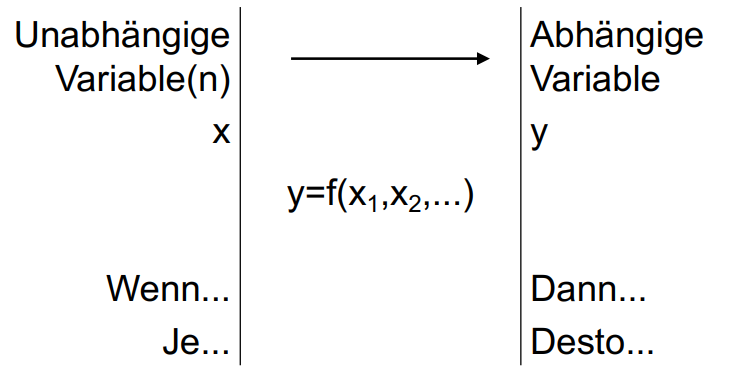
\includegraphics[keepaspectratio=true,height=7.5\baselineskip]{Hypothese.png}
	\caption{Hypothese}
	\label{fig:hypothese}
\end{wrapfigure}

Nebenstehende Abbildung (Abb. \ref{fig:hypothese}) veranschaulicht das Grundgerüst einer Hypothese. \\
Am Beispiel von 'Je reicher ein Staat, desto demokratischer ist er':

\begin{equation}
Demokratie_{Staat} = f(Reichtum_{Staat})
\end{equation}

Die unabhängige (oder auch erklärende/exogene) Variable ist der Reichtum des Staates und die abhängige (oder auch zu erklärende/endogene) Variable ist die Demokratisierung dieses Staates. Eine Hypothese kann beliebig viele unabhängige/exogene Variablen besitzen/vergleichen.



\subsection{Politik}
Der Begriff 'Politik' ist folgendermassen definiert:

\begin{quote}
    \blockquote{Soziales Handeln, das auf Entscheidungen und Steuerungsmechanismen ausgerichtet ist, die allgemein verbindlich sind und das Zusammenleben von Menschen regeln.}
\end{quote}

Die Politik lässt sich grundsätzlich in drei Arten unterteilen. In der Deutschen Sprache werden für alle drei Begriffe dasselbe Wort verwendet, im Englischen kann jedoch unterschieden werden zwischen: 
\begin{description}
    \item[Policy: ] \textit{Was} - Inhalte der Politik. Regeln, Weisungen
    \item[Polity:] \textit{Wer} - Die Strukturen und Akteure der Politik.  Organisationen, Parteien 
    \item[Politics:]  \textit{Wie} - Die Prozesse, wie Regeln, Weisungen etc. entstehen.
\end{description}

\subsection{Staat}
Ein Staat benötigt laut dem Völkerrecht mind. die folgenden drei Elemente, um als Staat anerkannt zu werden: 
\begin{description}
    \item[Staatsgebiet: ] Ein Gebiet, über welches der Staat die alleinige Macht hat
    \item[Staatsvolk: ] Ein Volk, welches im Staatsgebiet lebt und unter der Staatsgewalt des Staates ist.
    \item[Staatsgewalt: ] Der Staat hat das Recht, Gesetze zu erlassen und diese durchzusetzen. Er darf Steuern erlassen, um öffentliche Güter bereitzustellen oder Einkommen umzuverteilen. Jedoch muss der Staat die innere und äussere Sicherheit garantieren können.
\end{description}

\begin{figure}[htb]
    \centering
    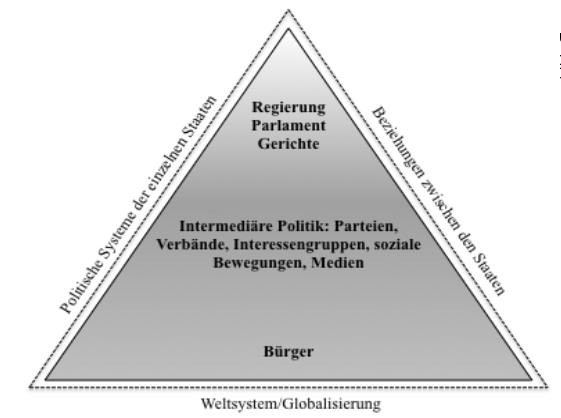
\includegraphics[keepaspectratio=true,height=10\baselineskip]{analytische_grundstruktur.png}
    \caption{Grundstruktur eines Staates}
    \label{fig:grundstrk_staat}
\end{figure}

Die Interessen der Staatsbürger werden meist über sogenannte \textit{Intermediärorgane} gewahrt. Das sind z.B. Parteien, Organisationan o.ä; Kurz gesagt, Polity.

\newpage

\section{Internationale Beziehungen}

Durch das Studium von internationalen Beziehungen versucht man zu verstehen, wie verschiedene Völker miteinander umgehen und miteinander auskommen. Die untersuchten Beziehungen können sowohl von freundschaftlicher, wie aber auch von kriegerischer Natur sein.

\vspace{10px}

Schimmelfennig beschreibt die internationale Politik als \blockquote[Schimmelfennig 2015, p.19]{Gesamtheit aller Interaktionen, die auf die autoritative Verteilung von Werten jenseits staatlicher Grenzen gerichtet sind}. Soll heissen; Alle Bemühungen, eine internationale Gesellschaft aufzubauen, die nach ähnlichen oder den gleichen Werten strebt.

\vspace{10px}

Im Gegensatz zur nationalen Politik, in welcher es eine Regierung in irgendeiner Form (Parlament, König o.ä) gibt, herrscht in der internationalen Politik \textbf{Anarchie}. Es gibt \textbf{keine zentrale Autorität} im internationalen System. Jegliche Allianzen und Kooperationen die zwischen Staaten existieren sind selbstbestimmt. Sie bleiben nur solange bestehen, wie der stärkere der beiden Staaten einen Gewinn daraus ziehen kann.

Diese Anarchie im internationalen Umfeld stellt die einzelnen Staaten je nach dem vor schwer zu lösende Probleme. Prinzipiell sind es dieselben Probleme, die sie auch staatsintern zu meistern haben, jedoch herrscht dort keine Anarchie (oder sollte zumindest nicht)

Grundsätzlich lassen sich diese Probleme in drei Hauptkategorien unterteilen:


\begin{description}
	\item[Sicherheit: ] Es gibt keine zentrale Autorität, die das Gewaltsmonopol hat, wie das in der inneren Politik der Fall ist. Jeder Staat muss selbst für seine Sicherheit sorgen.
	
	
	Das heisst, entweder findet ein Wettrüsten a la Kalter Krieg statt, oder aber man muss Allianzen eingehen. Diese Allianzen halten aber auch nur so lange, wie der stärkere Allianzpartner etwas davon hat.
	\item[Wohlfart: ] Aufgrund dessen, dass es keine zentrale Autoritätsstelle 	gibt, sind die internationalen Märkte enorm fragmentiert. Jeder Staat ist auf seinen eigenen Vorteil bedacht. Es werden nationale Währungen herausgegeben, Zölle für Import und Export erhoben und der grenzüberschreitende Warenaustausch wird von beiden Staaten streng überwacht. \\
	All das lässt sich mit einem Wort zusammenfassen: \textit{\textbf{ineffizient}}. Es gibt einen enormen bürokratischen Overhead und treiben die Preise in die Höhe, da die ganze Bürokratie irgendwie finanziert werden müsste.
	
	
	Im schlimmsten Fall kann dies zu Marktversagen führen. Marktversagen tritt dann auf, wenn Angebot und Nachfrage nicht mehr im Verhältnis stehen und somit zu massiv niedrigeren Preisen verkauft werden muss und somit Verluste eingefahren werden.
	
	\item[Freiheit: ] Die Bürger und Bürgerinnen eines jeden Staates geniessen gewisse Freiheiten innerhalb ihres Staates (idealerweise Meinungsfreiheit, Freiheit vor Folter, Verfolgung etc.). Diese Freiheiten sind jedoch an ihren jeweiligen Heimatstaat gebunden.
	
	
	Diese Freiheiten können sich je nach Herrschaft eines Staates enorm unterscheiden (man denke an die Unterschiede Schweiz vs. Nordkorea). Es müssen also Abmachungen getroffen und Verträge ausgehandelt werden, dass die Bürger aller Staaten in allen anderen Staaten vergleichbare Rechte geniessen.
\end{description}

\newpage

\section{Realismus und Neo-Realismus}

Der Realismus entstand in den 1930er Jahren als Reaktion auf \textit{das Scheitern des Völkerverbundes} und der \textit{aggressiven und expansiven Politik Japans, Italiens und Deutschlands}.

\vspace{10px}

\noindent Das realistische Staatensystem ist anarchistisch und die Nationalstaaten handeln selbstständig, stets mit dem Interesse des eigenen Staates im Hintergrund.

\vspace{10px}

\noindent Der Realismus basiert auf drei Hauptaussagen:

\begin{itemize}
	\item Der Mensch ist zerstörerisch und nicht vertrauenswürdig
	\item Ein Staat muss Macht besitzen, um sich im anarchischen Staatensystem durchsetzen zu können.
	\item Der Güterzuwachs eines Staates geht immer zulasten eines anderen Staates $\rightarrow$ Nullsummenspiel
\end{itemize}

Kooperationen/Bündnisse werden im Realismus nur sehr selten geschlossen und existiert nur so lange, wie der mächtigste Bündnispartner einen Gewinn daraus zieht. Lohnt sich das Bündnis für die Grossmacht nicht mehr, kündigt sie die Kooperation auf und die schwächere Macht kann nichts dagegen tun. Das Bündnis zerfällt ebenfalls, sobald die Macht der Grossmacht zerfällt.

Internationale Organisationen haben keine Macht per se, sie spiegeln nur die Machtverhältnisse der Mitglieder wieder (Die politische Stossrichtung der Grossmacht/des Hegemons diktiert die politische Stossrichtung der Organisation). 

\vspace{10px}

\noindent Die Stabilität einer solchen Organisation hängt von der Machtverteilung innerhalb der Organisation:

\begin{description}
	\item[Unipolar: ] Eine Grossmacht $\rightarrow$ Sehr stabil, ausser wenn die Grossmacht herausgefordert wird
    \item[Bipolar: ] Zwei oppositionelle Grossmächte $\rightarrow$ Stabil, da beide Grossmächte meiteinander im Wettkampf stehen (siehe Kalter Krieg Abb.  \ref{fig:bipolaritaet})
	\item[Multipolar: ] Konstanter Machtkampf $\rightarrow$ Instabil.
\end{description}

\begin{figure}[htb]
    \centering
    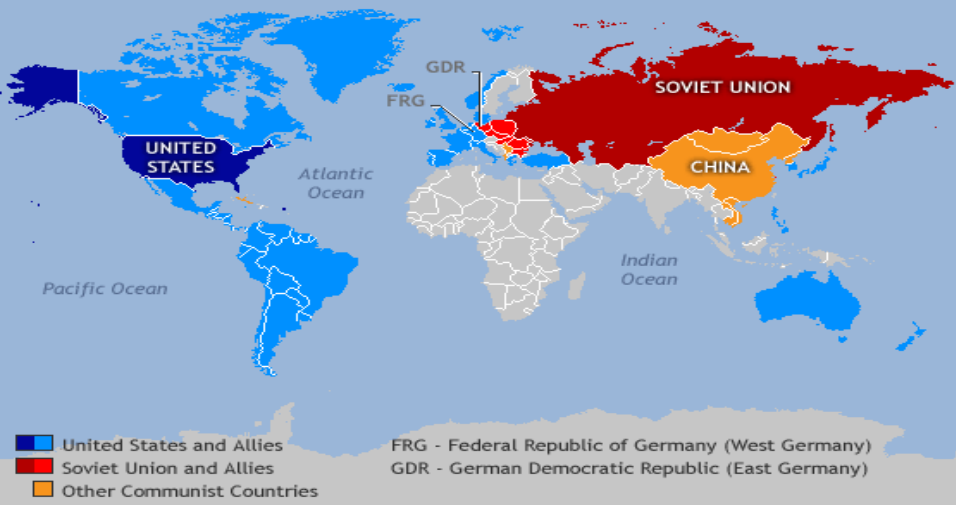
\includegraphics[keepaspectratio=true,height=15\baselineskip]{bipolaritaet.png}
    \caption{Bipolarität des kalten Krieg}
    \label{fig:bipolaritaet}
\end{figure}

Da das internationale Staatensystem immer noch anarchistisch ist, streben die einzelnen Staaten nach möglichst viel Macht, um sich in dieser Umgebung behaupten zu können. \textbf{Macht ist somit das oberste Gut}. Erst wenn der Staat genügend Macht besitzt, um Sicherheit garantieren zu können, kann er sich um weitere Dinge wie z.B. Wohlstand und Freiheit kümmern.

\subsection{Gefangenendilemma}

\begin{figure}[htb]
    \centering
    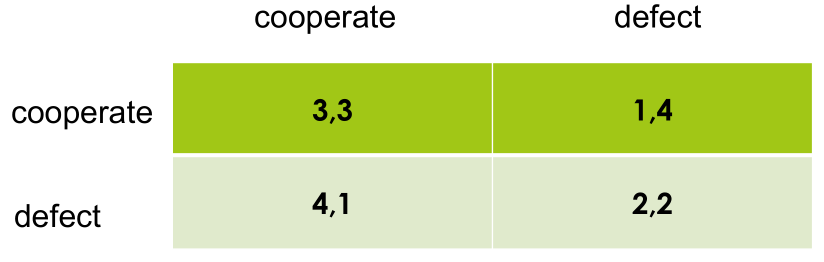
\includegraphics[keepaspectratio=true,height=10\baselineskip]{gefangenendilemma.png}
    \caption{Darstellung des Gefangenendilemmas}
    \label{fig:gefangenendilemma}
\end{figure}

Viele politische Entscheidungen im Realismus folgen der Denkweise des Gefangenendilemmas. Das Dilemma lautet

\begin{quote}
	Zwei Gefangene werden getrennt verhört. Man hat noch keine Beweise gegen sie in der Hand. Die Gefangenen haben die Möglichkeit zu kooperien und damit straffrei davonzukommen aber den Partner zu verraten (cooperate) oder aber nicht zu kooperieren (defect) und die Strafe selbst abzusitzen 
\end{quote}



Das optimale Vorgehen wäre es, wenn niemand kooperieren würde und somit beide 2 Jahre absitzen muss. Jedoch sind Menschen misstrauisch und vertrauen nicht darauf, dass ihr Partner sie nicht verratet um straffrei davonzukommen (Szenario cooperate/defect oder andersrum). Somit sieht die Realität meist so aus, dass beide kooperieren und somit beide 3 Jahre absitzen müssen.

\newpage

\section{Insititutionalismus}

Der heute verbreitetere Insititutionalismus ist der sog. \textbf{Neoliberae (rationalistische) Insititutionalismus}, der auf einer \textit{zivilisierten Anarchie} aufbaut. Das heisst, im internationalen Staatenverbund herrscht zwar immer noch Anarchie, jedoch haltet man sich doch an gewisse Regeln.

Im Gegensatz zum Realismus streben die Staaten im Insititutionalismus nicht nach Macht, sondern nach \textbf{Wohlstand}. Das heisst, Staaten arbeiten aktiv miteinander (Kooperation), um zusammen den höchstmöglichen Gewinn zu erwirtschaften. Dies führt zu einer \textbf{Interdependenz}, einer gegenseitigen Abhängigkeit. 

Auch Hegemone wie die USA oder China sind nicht ausgeschlossen von dieser Interdependenz. Man stelle sich vor, die gesamte Welt würde China boykottieren. Sicherlich hätte dies auch katastrophale Folgen für die westliche Wirtschaft, jedoch wäre China alleine auch nicht überlebensfähig, da ein grosser Teil von Chinas Wohlstand vom Export kommt.

Es findet also eine Verschiebung der Macht statt. Anstelle von militärischer Macht wird nun wirtschaftliche Macht angestrebt.

\subsection{Schatten der Zukunft} \label{sec:sdz} 
Der Schatten der Zukunft beschreibt ein Aspekt des Gefangenendilemmas (Abb. \ref{fig:gefangenendilemma}). Der Schatten der Zukunft ist die Wahrscheinlichkeit, mit welcher beide Parteien später wieder aufeinandertreffen könnten. Viele Entscheidungen im Insititutionalismus werden durch Reziprozität getroffen: \textit{Wenn du deine Grenzen für den Handel öffnest, dann mach ich das auch. Aber nur dann}. Je wahrscheinlicher es ist, dass beide Parteien später wieder aufeinander treffen könnten, ergo wieder voneinander profitieren könnten, desto kooperativer verhalten sie sich (denn man will ja den Gegenüber nicht vergraulen und sich somit eventuelle spätere Gewinne durch die Lappen gehen lassen). Wenn der Schatten der Zukunft jedoch klein oder sogar nonexistent ist, so sind beide Parteien wieder ausschliesslch auf das eigene Wohl bedacht und werden eher 'defect' wählen.

\vspace{10px}

\noindent Ein wichtiger Aspekt des Schattens der Zukunft sind \textbf{internationale Organisationen} (oder Regimes (Kap. \ref{sec:Regime}))  wie die UNO, die WTO oder ähnliches. Solche internationalen Organisationen vergrössern den Schatten der Zukunft enorm.

\vspace{10px}

\noindent IOs haben zahlreiche Vorteile für alle Beteiligten:

\begin{itemize}
    \item Vergrössert Schatten der Zukunft
    \item Verringert Transaktionskosten
    \item Verringert Unsicherheit
    \item Ermöglicht abgesicherte Verpflichtungen
    \item Informationsaustausch
    \item Ermöglicht monitoring und Sanktionen falls nötig
\end{itemize}
\newpage
\subsection{Realismus vs. Insititutionalismus}

\begin{figure}[htb]
    \centering
    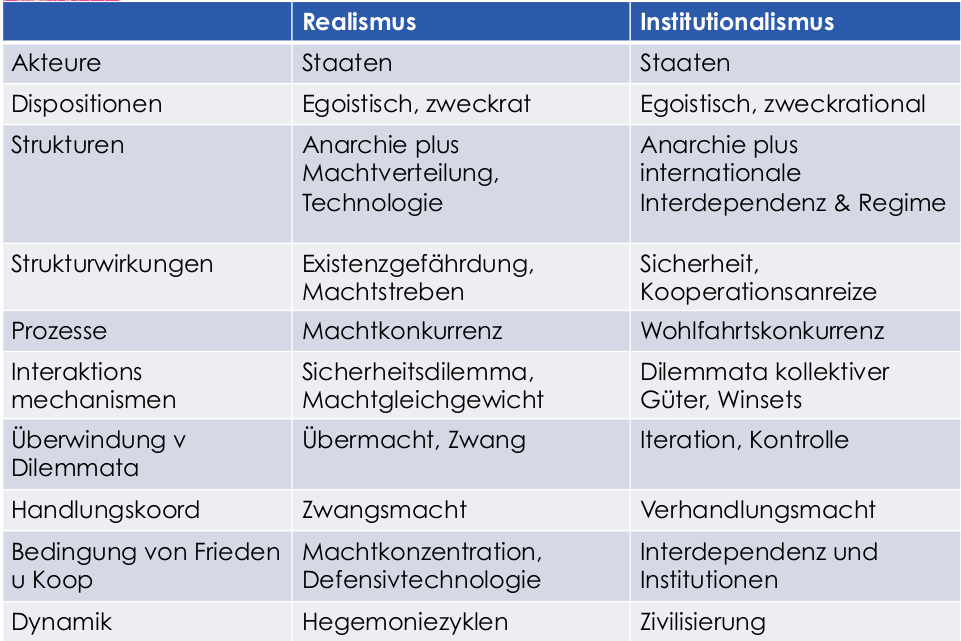
\includegraphics[keepaspectratio=true,height=20\baselineskip]{realismusvsinstitutionalismus.png}
    \caption{Gegenüberstellung von Realismus und Insititutionalismus}
    \label{fig:realismusvsinstitutionalismus}
\end{figure}

\section{Transnationalismus}
\begin{quote}
	\blockquote[Kernhypothese des Transnationalismus]{Je dichter und symmetrischer die transnationale Verflechtung im internationalen System ist, desto höher ist die Wahrscheinlichkeit von Frieden und Internationaler Kooperation}
\end{quote}


Der Transnationalismus setzt auf Handel als Strategie zur Sicherung des Friedens und zur Mehrung des internationalen Wohlstandes.

Oberhäupte sind internationale Organisationen oder 'Transnationale Netzwerke' (anstelle von Regierungen). Solche Netzwerke bilden sich hauptsächlich, wenn die internationale Politik keinen Konsens oder keine Lösung findet. 

\begin{figure}[htb]
	\centering
	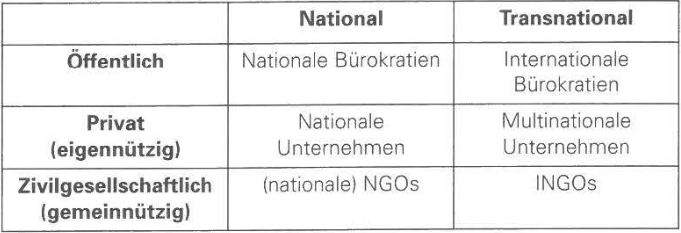
\includegraphics[keepaspectratio=true,height=10\baselineskip]{akteureTransnationalismus.png}
	\caption{Akteure des Transnationalismus}
	\label{fig:akteureTransnationalismus}
\end{figure}

\noindent Im Gegensatz zu bisher besprochenen Bewegungen streben die Akteure des Transnationalismus weder nach Macht (Realismus), noch nach Wohlfahrtsgewinn (Institutionalismus). 

Akteure können grundsätzlich an drei Dingen interessiert sein:

\begin{itemize}
	\item Am Nutzen von anderen $\rightarrow$ Altruistisch
	\item Am Nutzen des Kollektivs $\rightarrow$ Gemeinnützig
	\item An Ideen und Werten $\rightarrow$ Idealistisch
\end{itemize}

\noindent Aufgrund der internationalen Vernetzung durch internationale Organisationen werden die Probleme der Unsicherheit und der Anarchie massiv gedämpft.

\vspace{10px}

\noindent Transnationale Netzwerke bilden sich vor allem dann, wenn internationale Lösungen gescheitert sind. Man nehme das Beispiel von Ebola in Westafrika: Die WHO (eine internationale Organisation) rief den Notstand viel zu spät aus ($\rightarrow$ scheiterte). Die MSG (ein transnationales NGO) griff ein und machen einen Grossteil der zu erledigenden Arbeiten.

\begin{figure}[htb]
	\centering
	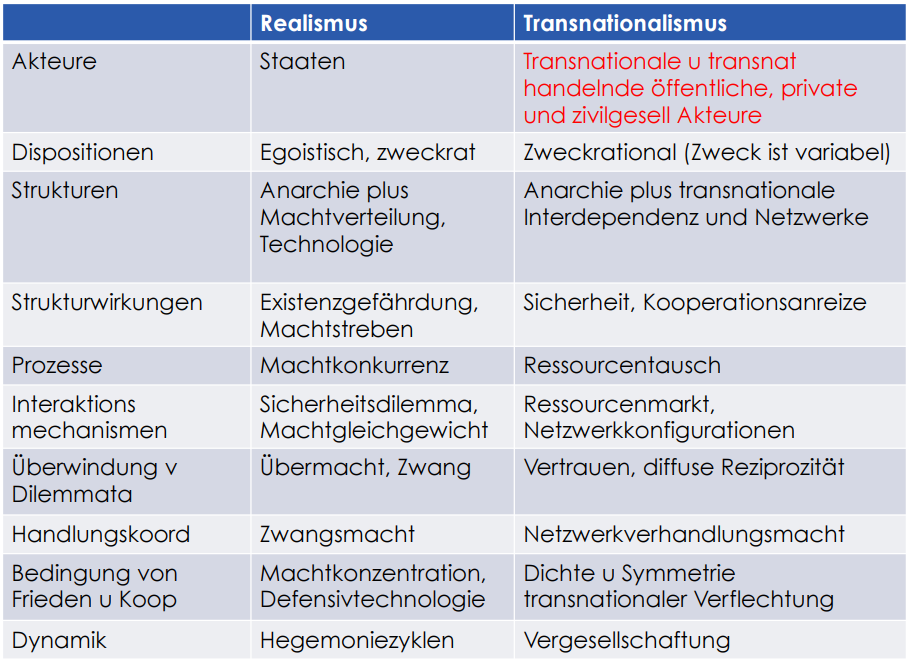
\includegraphics[keepaspectratio=true,height=20\baselineskip]{RealismusVsTransnationalismus.png}
	\caption{Realismus vs. Transnationalismus}
	\label{fig:realismusvstransnationalismus}
\end{figure}


\section{Liberalismus}
\begin{quote}
	\blockquote[Ziel des Liberalismus]{Herstellung einer internationalen Friedensordnung (Weltfrieden), einer besseren Welt; Kooperation und Interessenausgleich im Netzwerk internationaler und transnationaler Organisationen}
\end{quote}

\vspace{10px}

\noindent Nach Kant müssen für den Weltfrieden drei Bedingungen erfüllt sein:

\begin{itemize}
	\item Demokratie
	\item Internationales Recht/Organisationen
	\item Interdependenz/Gegenseitige Abhängigkeiten von Staaten
\end{itemize}

\noindent Der Liberalismus strebt danach, den Akteur 'Staat' aufzusplitten in innerstaatliche Akteure mit eigenen Zielen und Machtverhältnisse untereinander. Diese 'Subakteure' beeinflussen dann die Kooperationsbereitschaft der einzelnen Staaten. 

Der Staat agiert zwar immer noch als ausserpolitisches Handlungsorgan der Gesellschaft, sein Wirken wird jedoch von diesen internen Subakteuren bestimmt.

Aufgrund dessen, dass liberaldemokratische Staaten prinzipiell friedliebend und kooperationsbereit sind, kann gesagt werden dass \textit{je höher die Anzahl liberaldemokratischer Staaten im internationalen System, desto höher ist die Wahrscheinlichkeit von Frieden und Kooperation}.

\vspace{10px}

\noindent Bei Verhandlungen auf internationaler Ebene werden im Liberalismus meist sog. "Two Level Games" gespielt: Der Abgesandte des Staates mag zwar ein Ergebnis der Verhandlung unterschreiben, jedoch muss diese Entscheidung erst noch staats-intern abgesegnet werden (z.B. durch das Parlament oder die Wähler).

\begin{figure}[htb]
	\centering
	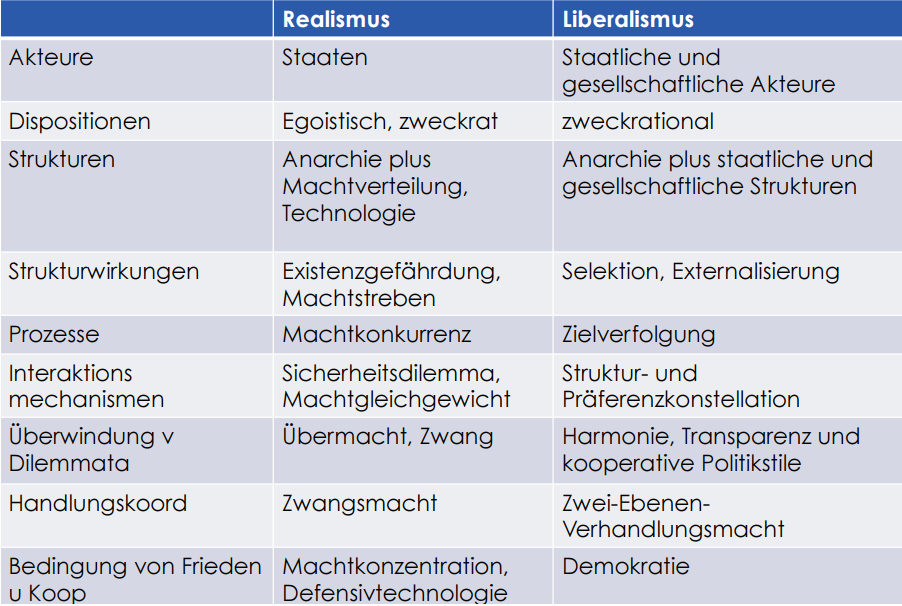
\includegraphics[keepaspectratio=true,height=20\baselineskip]{RealismusVsLiberalismus.png}
	\caption{Realismus vs. Liberalismus}
	\label{fig:realismusvsliberalismus}
\end{figure}

\section{Konstruktivismus}
\begin{quote}
	\blockquote[Konstruktivismus]{Je grösser die Übereinstimmung der Ideen von internationalen Akteuren und je stärker damit die Gemeinschaft zwischen ihnen ist, desto höher ist die Wahrscheinlichkeit von Frieden und internationaler Kooperation}
\end{quote}

\noindent Der Konstruktivismus ist das Gegenstück zu rationalistischen und materiellen Sichtweisen. Die Akteure sind weder an der militärischen noch an der ökonomischen Macht ihres Gegenübers interessiert, sondern basieren ihre Entscheidungen und Handlungen ausschliesslich auf den Normen, Werten und Ideen des Gegenübers. So könnte zum Beispiel ein sehr gewinnbringender Deal zwischen zwei Staaten abgeblasen werden, da sie nicht dieselben Wertvorstellungen haben.

\vspace{10px}

\noindent Kooperationen im Konstruktivistischen Umfeld sind meist sehr stabil, da sie auf gemeinsamen Überzeugungen beruhen und schon fast als Freundschaften bezeichnet werden können. 

Dem gegenübergestellt sind 'Feindschaften'. Der andere wird als Gegensatz definiert; Jemand, der nicht dieselben Wertvorstellungen hat und somit nicht als Kooperationspartner nicht in Frage kommt. 

\vspace{10px}

\noindent Das Gefangenendilemma (vgl. \ref{fig:gefangenendilemma}) wird somit mehr oder weniger aus der Welt geschafft, da Freunde stets 'cooperate' wählen werden, während Feinde stets 'defect' wählen.

\noindent Akteure handeln Sozial, intersubjektiv und normativ:

\begin{description}
	\item[Sozial: ] Verhalten und Entscheidungen gemäss der 'Richtigkeit' (sozial angemessen) unabhängig von eventuellen Kosten und erwarteten Nutzen.
	\item[Intersubjektiv: ] Einbeziehung der Verhaltenserwartungen anderer Akteure
	\item[Normativ: ] Verfolgung sozialer und normativer Interessen, die sich endogen herausbilden und durch Interaktionen und kommunikative Prozesse veränderbar sind.
\end{description}

\noindent Institutionen im Konstruktivismus haben eine strukturierende Wirkung: Sie lehren die Akteure und beeinflussen somit deren Identität, Präferenzen und Einstellungen.

Zudem haben sie institutionsintern spezielle Normen, Regeln und Verfahren.

\paragraph{Sozialisation} \mbox{} \\
Internationale Sozialisation ist der Prozess, bei dem Akteure dazu gebracht werden, die Ideen und Identität einer international Gemeinschaft zu übernehmen und zu reproduzieren. 

\begin{figure}[htb]
	\centering
	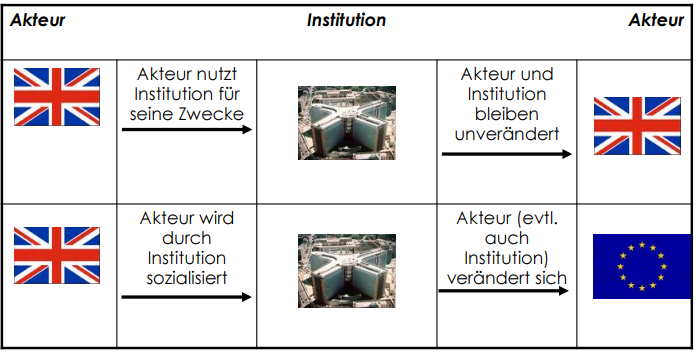
\includegraphics[keepaspectratio=true,height=15\baselineskip]{sozialisation.png}
	\caption{Beispiel von internationaler Sozialisation}
	\label{fig:sozialisation}
\end{figure}

\begin{landscape}
	\begin{figure}[htb]
		\centering
		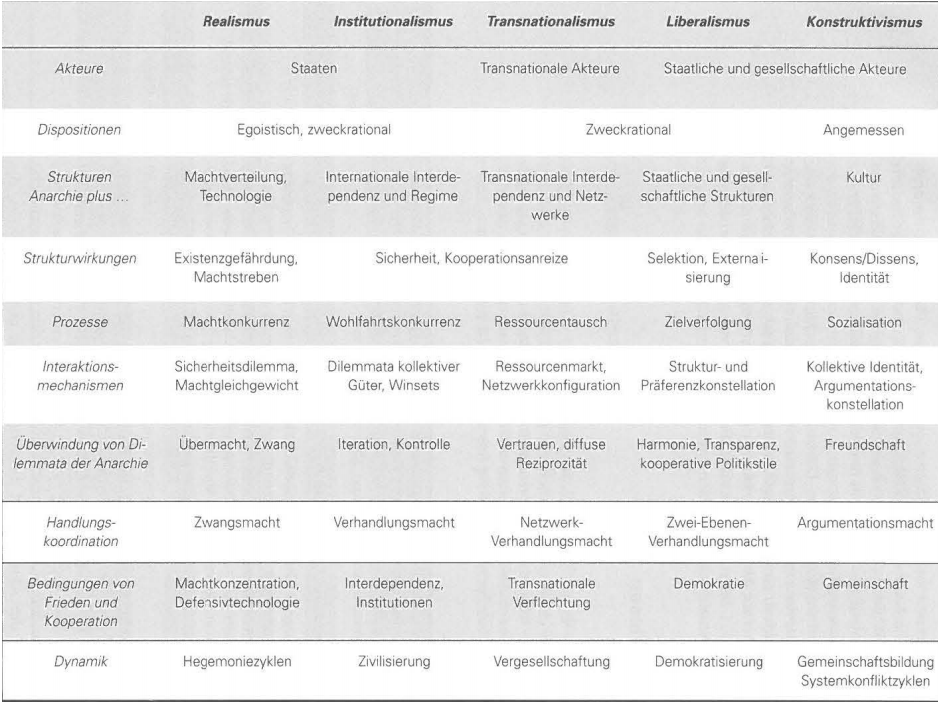
\includegraphics[keepaspectratio=true,height=30\baselineskip]{Gegenueberstellung.png}
		\caption{Gegenüberstellung der einzelnen behandelten Grosstheorien}
		\label{fig:gegenueberstellung}
	\end{figure}
\end{landscape}

Zusammengefasst kann gesagt werden, Entscheidungen im der internationalen Politik werden anhand von 7 Faktoren getroffen:

\begin{description}
	\item [Macht] Ressourcenverteilung, Polarität und Hegemonie
	\item [Technologie]
	\item [Interdependenz] Art, Stärke und Symmetrie
	\item [Internationale Institutionen] Existenz, Stärke
	\item [Netzwerke] Beteiligte, Dichte und Zentralität
	\item [Subsystemische Strukturen] Machtverteilung, Institutionen, internationale Kompatibilität
	\item [Kultur] Ideen, Wertvorstellungen und Identitäten
\end{description}

\hrulefill

\vspace{10px}

\noindent \textbf{Dies ist das Ende der Zusammenfassung der Grosstheorien. Von nun an werden die sog. 'Mid-level theories' behandelt}

\vspace{10px}

\hrulefill

\vspace{30px}

\noindent Grosstheorien machen Aussagen über Akteure, Interaktionen und Outcomes von Begegnungen in internationalen Beziehungen. Mid-range oder Mid-Level Theorien sind nicht ganz so abstrakt wie Grosstheorien, sondern befassen sich mit kleineren Phänomenen der internationalen Politik

\newpage

\section{Regime / Internationale Organisationen} \label{sec:Regime}
\begin{quote}
	\begin{blockquote}[Krasner 1983]{Regimes are sets of implicit or explicit principles, norms, rules and decision-making procedures around which actors' expectations converge in a given area of international relations'}
	\end{blockquote}
\end{quote}

\noindent Krasner beschreibt Regimes also als viergliedrige Struktur:

\begin{description}
	\item[Principles: ] Theoretische Aussagen darüber, wie man die Welt versteht \\
	\textit{Globale Wohlfahrt wird durch Handel maximiert}
	\item[Norms: ] Generelle Verhaltensstandards, Rechte und Pflichten von Mitglieder \\
	\textit{Zölle und Handelshemmnisse sollten möglichst reduziert und schlussendlich abgebaut werden}
	\item[Rules:] Mehr oder weniger dasselbe wie Principles, jedoch weniger generell gehalten \\
	\textit{z.B. diese Principles gelten nur für Entwicklungsländer}
	\item[Decision-making procedures: ] Spezifische Vorschriften, die die Entscheidungsfindung regeln. 
	\textit{Die Stimme von Staaten mit >10M Einwohner zählt doppelt}
\end{description}

\noindent Eine weitere, oft zitierte Definition eines Regimes kommt von Stein:
\begin{quote}
	\begin{blockquote}[Stein 1982]{A regime exists when the interaction between the parties is not unconstrained or is not based on independent decision making}
	\end{blockquote}
\end{quote}

\noindent Ein bisschen verständlicher erklärt das Wikipedia: 
\begin{quote}
	\begin{blockquote}[Wikipedia]{Internationale Regime sind \textbf{kooperative Institutionen}, die durch informelle und formelle, rechtliche und nichtverrechtlichte Strukturen gekennzeichnet sind und \textbf{Konflikte zwischen Nationalstaaten bearbeiten}. Sie sollen die Transaktionskosten reduzieren und ein \textbf{beidseitiges Geben und Nehmen für alle Beteiligten bewirken}. Zwar vertrauen sich die Staaten immer noch nicht, aber durch Kontrollen innerhalb der Regime soll dem entgegenzuwirken versucht werden.}
	\end{blockquote}
\end{quote}
Ein Beispiel eines internationalen Regimes ist z.B. die UNO oder die WTO. Sie sind Staaten-unabhängige Instanzen, die als Mediator agieren können. Durch Regimes kann auch die Effizienz erhöht werden. Man nehme das Beispiel der bilateralen Verträge der Schweiz. Es wäre ein enormer Aufwand für die Schweiz sicherzustellen, dass alle Vertragsklauseln eingehalten werden. Stattdessen übernimmt dies eine unabhängige Instanz ($\rightarrow$ Regime).  


\vspace{10px}

Regimes werden oft zur Streitschlichtung beigezogen, da sie unabhängig und zentral sind. Keiner der beiden Parteien hat einen unfairen Vorteil gegenüber der anderen Partei.

\subsection{Gründe}

\subsubsection*{Zentralisierung}

Internationale Organsiationen bieten eine stabile Organisationsstruktur mit einer eigenen Bürokratie, die gemeinschaftlich Aktivitäten unternimmt. Die innerstaatliche Bürokratie der einzelnen Delegierten wird (idealerweise) an der Tür zurückgelassen

\paragraph{Vorteile} \mbox{}\\

\begin{itemize}	
	\item Klar definierte Entscheidungsstrukturen $\rightarrow$ Schnelle Entscheidungen
	\item Stabiles/spezialisiertes Forum für wiederholte Verhandlungen
\end{itemize}

\textbf{$\rightarrow$}  Bessere zwischenstaatliche Interaktion \textbf{$\rightarrow$}  effizientere internationale Zusammenarbeit.

\begin{itemize}
	\item Pooling von Aktivitäten, Ressourcen und Risiken
	\item Gemeinsame "Produkte" und Projekte
	\item Schaffung von Prozeduren für die konkrete Ausarbeitung Normen, Regeln und Standards
\end{itemize}

$\rightarrow$  Übernahme von gemeinsamen Aufgaben und Aktivitäten $\rightarrow$  Bessere zwischenstaatliche Interaktion.

\subsubsection*{Unabhängigkeit}

Innerhalb eines klar definierten Rahmens kann und darf eine Internationale Organisation autonom (unabhängig) handeln

\paragraph{Vorteile} \mbox{}\\

\begin{itemize}
	\item Legitimes Handeln durch unabhängige Organisation
	\item Neutralität als Informationsbeschaffer, Verteiler, Treuhänder und Schiedsrichter
\end{itemize}

\textbf{$\rightarrow$} Effizienteres Handeln / Bessere Interaktion untereinander

\subsection{Staaten <> Internationale Organisationen}

Es gibt gewisse Mechanismen, wie sich Staaten und IOs gegenseitig beeinflussen können.

\subsubsection{Two-Level games vs. Locking-In}

\paragraph{Two-Level Games} \mbox{}\\
Das two-level game ist eine beliebte Strategie von Delegierten bei Verhandlungen: Der Delegierte stimmt dem Ergebnis zu, merkt aber an, dass es nicht rechtskräftig ist, bis es durch die heimische Regierung gegangen und akzeptiert wurde (z.B. Parlament, Stimmvolk etc.). So kann das Ergebnis zwar angenommen werden, jedoch ist es trotzdem nicht ganz angenommen.

\paragraph{Locking-in} \mbox{}\\
Beim Locking-In verhält es sich genau andersherum. Ein Delegierter (oder das Staatsoberhaupt) kommt zurück in die Heimat mit einem Beschluss, den er bereits als rechtskräftig durchsetzt mit der Begründung, dass das so in der Versammlung der IO beschlossen wurde und dieser Staat somit diesem Beschluss 'Folge leisten müsse'.

\vspace{10px}

\noindent Beide diese Technologien funktionieren jedoch nur dank der Zentralisierung der IOs (Two-Level-Games) und deren Unabhängigkeit (Locking-In)

\section{Analyse von politischen Events}

Bei der Analyse von politischen Handlungen müssen immer mind. drei Dinge geklärt werden:

\begin{description}
	\item[Interessen: ] Was wollen die Akteure?
	\item[Interaktionen:] Warum können sie es nicht bekommen?
	\item[Institutionen: ] Spielen Regeln eine Rolle für die Weltpolitik?
\end{description}

\subsection{Interessen}
Interessen können in drei Hauptkategorien fallen:

\begin{itemize}
	\item Macht/Sicherheit $\rightarrow$ Realismus
	\item Ökonomische/materielle Wohlfahrt $\rightarrow$ Institutionalismus
	\item Ideologische Ziele wie z.B. religiöse $\rightarrow$ Konstruktivismus
\end{itemize}

\subsection{Interaktionen}
Die Interaktion beschreibt, wie die Entscheidungen de einzelnen Akteure sich beeinflussen und miteinander interagieren und somit ein Resultat oder ein politisches Outcome erzeugen.

\vspace{10px}

\noindent Die Entscheidungen der einzelnen Akteure hängt von ihrer ihren Strategien ab. Diese Strategien hängen wiederum von den Strategien der anderen Akteure ab. \\

Die Strategie ist ein Plan, sich so gut wie möglich zu positionieren, gegeben die Erwartungen bezüglich des Verhaltens und der Strategien anderer.

\vspace{10px}

\noindent Es gibt zwei Hauptkategorien von Interaktionen:
\begin{description}
	\item[Kooperation: ] Win - win Situation. Beide Akteure gewinnen
	\item[Verhandlung: ] Win - Lose Situation. Ein Akteur gewinnt die Verhandlung und steht letzten Endes besser da als der andere
\end{description}

Ob es zur Kooperation kommt, hängt meist von der Grösse und Macht de Akteure ab. Ebenfalls kommt es darauf, wer welche Informationen besitzt.

Kooperationen werden durch Institutionen beeinflusst, indem sie zum Beispiel sicherstellen, dass alle Parteien nach den Regeln spielen, Streite zwischen den Parteien schlichten und gewisse Verhaltensstandards sicherstellen.

\section{Internationale Politische Ökonomie}

\begin{center}
	\blockquote[Defintion von IPÖ]{Die Internationale Politische Ökonomie (IPÖ) untersucht die Wechselwirkung zwischen der (internationalen) Wirtschaft und der nationalen und internationalen Politik. \\}
\end{center}

Die IPÖ befasst sich hauptsächlich mit folgenden Themengebieten:

\begin{itemize}
	\item Internationalen Handel und Produktion
	\item Internationale Geld- und Finanzbeziehungen
	\item Internationale Zusammenarbeit in der Wirtschaftspolitik
	\item Weitere globale Phänomene, wie z.B. die Umwelt oder die Migration
\end{itemize}

\subsection{Vorteile von internationalem Handel}

Internationaler Handel hat einige Vorteile wie zum Beispiel:

\begin{itemize}
	\item Mehr Auswahl, Effizienz und niedrigere Preise durch vermehrter Wettbewerb.
	\item Steigerung des nationalen und globalen Wohlstands (da jeder mit jedem handelt)
	\item Grössere Wahrscheinlichkeit von Frieden (sog. 'Freihändlerischer Frieden' $\rightarrow$ 'Wenn wir im Krieg sind können wir nicht mehr mit ihnen handeln'
	\item Schnellere Verbreitung von Technologie ($\rightarrow$ Steigerung der Produktivität und wirtschaftlicher Entwicklung)
\end{itemize}

\subsection{Absoluter Vorteil vs. Komparativer Vorteil}

\begin{multicols}{2}
	\paragraph{Absoluter Vorteil} \mbox{} \\
	Es wird von absolutem Vorteil über eine Ware gesprochen, wenn ein Land diese Ware billiger/mit weniger Ressourcen herstellen kann als alle anderen.
\columnbreak
	\paragraph{Komparativer Vorteil} \mbox{}\\
	Der Komparative Vorteil ist eine Weiterentwicklung des absoluten Vorteils. Er besagt, dass Handel zwischen zwei Ländern auch vorteilhaft sein kann, wenn eines der beiden Länder den absoluten Vorteil über alle gehandelten Güter hat.
\end{multicols}

Ein Beispiel des komparativen Handels geklaut von Wikipedia:

\vspace{10px}
\begin{wraptable}{r}{0.6\textwidth}
	\begin{tabular}{|c|c|c|}
		\hline
		\textbf{Tätigkeit} & \textbf{Nachbar A} & \textbf{Nachbar B} \\
		\hline
		Rasenmähen & 6h & 3h \\
		\hline
		Hecke Schneiden & 8h & 2h \\
		\hline
		\textbf{Benötigte Zeit} & \textbf{14h} & \textbf{5h} \\
		\hline
	\end{tabular}
\end{wraptable}

Nachbar A und Nachbar B müssen beide Gartenarbeit machen. Nachbar B ist zwar in allen Belangen besser als Nachbar A (zumindest was Gartenarbeit anbelangt). Jedoch können beide Parteien trotzdem noch Handel treiben, der für beide gewinnbringend ist.

\vspace{10px}

Nachbar A benötigt also 14h um seine Gartenarbeit zu erledigen, Nachbar B nur 5h. Obwohl Nachbar A in keiner der Gartenarbeit 'gut' ist (den absoluten Vorteil hat), so ist er trotzdem besser im Rasenmähen als im Hecken schneiden. 

\begin{wraptable}{L}{0.6\textwidth}
	\begin{tabular}{|c|c|c|}
		\hline
		\textbf{Tätigkeit} & \textbf{Nachbar A} & \textbf{Nachbar B} \\
		\hline
		Rasenmähen & 12h & - \\
		\hline
		Hecke Schneiden & - & 4h \\
		\hline
		\textbf{Eingesparte Zeit} & \textbf{2h} & \textbf{1h} \\
		\hline
	\end{tabular}
\end{wraptable}

\noindent Wenn sich die beiden Nachbarn nun absprechen (Handel betreiben) und Nachbar A die Arbeit übernimmt, die er ein bisschen besser kann (Rasen mähen) und Nachbar B die Andere, so können trotzdem beide Parteien Gewinn daraus schlagen.

\vspace{10px}

\subsection{Heckscher-Ohnlin Theorem}

Das Heckscher-Ohnlin Theorem befasst sich mit der Frage, welches der hergestellten Güter ein Land exportieren/handeln wird, wenn es nirgends einen absoluten Vorteil hat. 

Das Theorem besagt, dass das Land die Güter exportieren wird, die es vergleichsweise am billigsten herstellen kann. "Billig" heisst in dem Fall, dass die Herstellung des Gutes hauptsächlich Ressourcen benötigt, die im Land reichlich vorhanden sind. 

Dafür wird das Land diese Güter importieren, deren Herstellung hauptsächlich Ressourcen benötigt, die das Land nicht reichlich vorhanden sind.
\vspace{10px}

\noindent 'Ressourcen' sind in diesem Fall entweder Kapital oder Arbeit. Das heisst also, dass ein Land, das viel Kapital hat Güter die viel Arbeit bei der Herstellung benötigen importieren wird und dafür Güter, die teuer sind in der Herstellung exportieren. Bei einem Land, das viele Arbeitskräfte, jedoch wenig Geld hat wird es genau umgekehrt sein. 

\subsection{Stolper-Samuelson Theorem}
Das Stolper-Samuelson Theorem besagt, dass nach der Verteuerung eines Gutes die Entlohnung desjenigen Produktionsfaktors steigt, der am Meisten benötigt wird in der Produktion des Gutes.

\subsection{Protektionismus}

Protektionismus beschreibt die staatliche Intervention zum Schutz der eigenen Wirtschaft z.B. durch das künstliche Erhöhen der Importzölle um Importe niedrig zu halten.


\end{document}
